% =====================================================================
% schema_saga.tex — Schema SAGA (Defazio, Bach & Lacoste-Julien, 2014)
% Stesso codice TikZ dell'Appendice "Schemi dei metodi a varianza
% ridotta" della tesi (fig:saga). Compilare con pdflatex.
% =====================================================================
\documentclass[border=8pt]{standalone}
\usepackage[T1]{fontenc}
\usepackage[utf8]{inputenc}
\usepackage{amsmath, amssymb}
\usepackage{tikz}
\usetikzlibrary{arrows.meta, positioning, calc}
\definecolor{coverblue}{RGB}{30, 60, 120}

\begin{document}
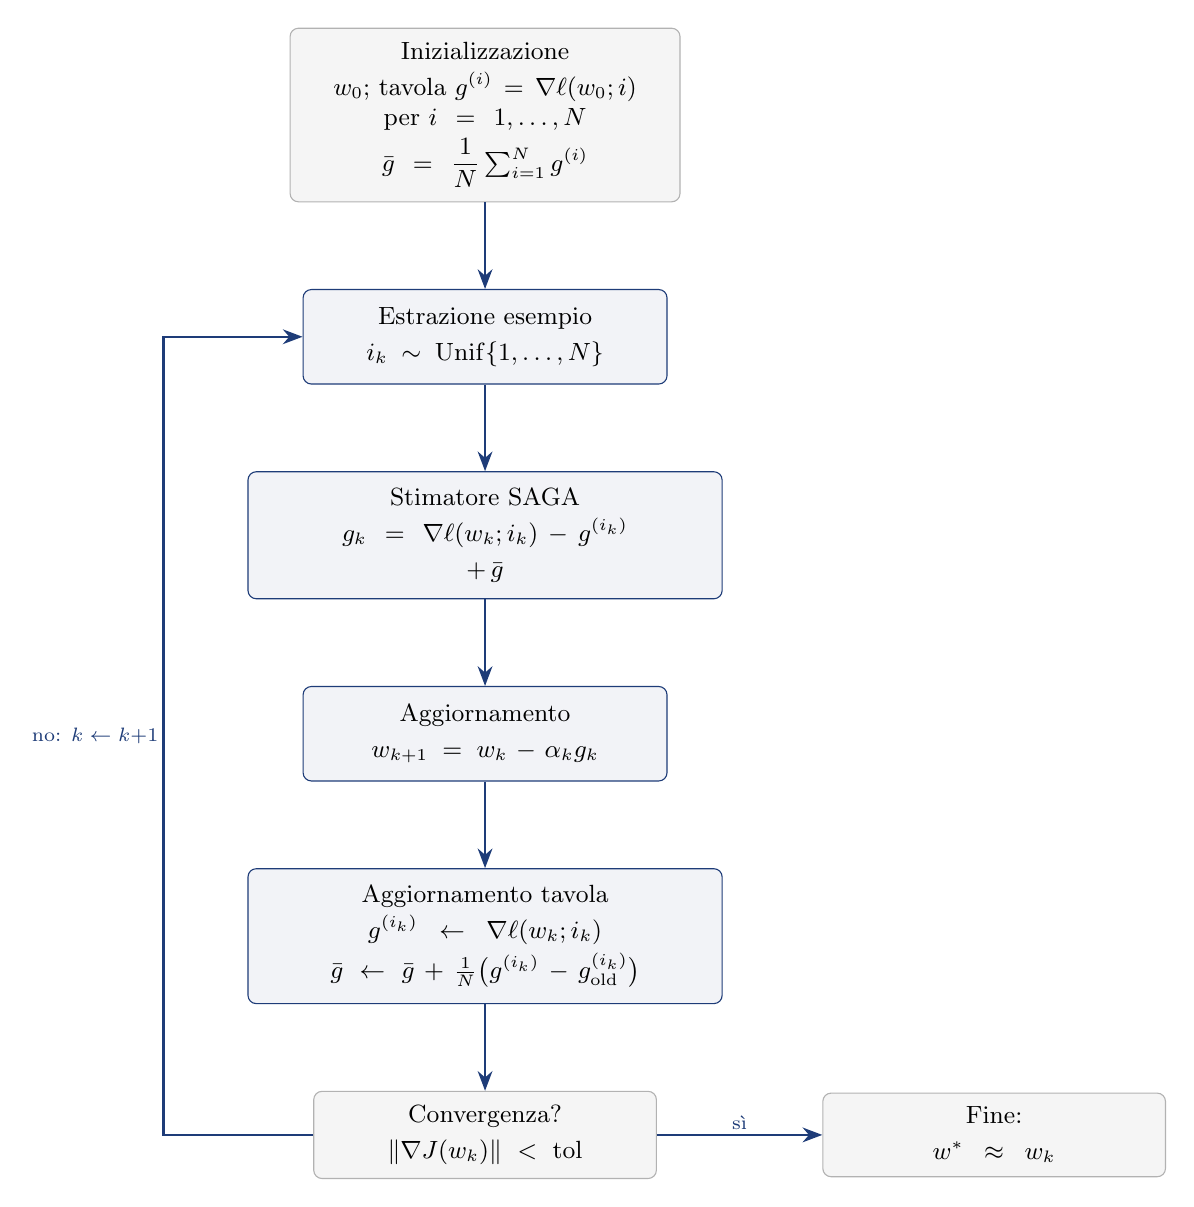
\begin{tikzpicture}[
  node distance=1.1cm and 2.4cm,
  every node/.style={font=\small},
  box/.style={
    draw=coverblue, fill=coverblue!6, rounded corners=3pt,
    text width=4.2cm, align=center, minimum height=1.2cm,
    inner sep=6pt
  },
  io/.style={
    draw=gray!60, fill=gray!8, rounded corners=3pt,
    text width=4.0cm, align=center, minimum height=1.0cm,
    inner sep=5pt
  },
  arrow/.style={-{Stealth[length=2.5mm]}, thick, color=coverblue},
  label/.style={font=\scriptsize, fill=white, inner sep=1.5pt}
]

  % Nodi principali (colonna centrale)
  \node[io, text width=4.6cm, minimum height=1.6cm] (init) {Inizializzazione\\[2pt] $w_0$; tavola $g^{(i)} = \nabla\ell(w_0; i)$ per $i = 1,\dots,N$\\[2pt] $\bar g = \dfrac{1}{N}\sum_{i=1}^{N} g^{(i)}$};
  \node[box, below=of init] (estrai) {Estrazione esempio\\[2pt] $i_k \sim \mathrm{Unif}\{1,\dots,N\}$};
  \node[box, below=of estrai, text width=5.6cm, minimum height=1.6cm] (stim) {Stimatore SAGA\\[2pt] $g_k = \nabla\ell(w_k; i_k) - g^{(i_k)}$\\[2pt] $+ \, \bar g$};
  \node[box, below=of stim] (agg) {Aggiornamento\\[2pt] $w_{k+1} = w_k - \alpha_k g_k$};
  \node[box, below=of agg, text width=5.6cm, minimum height=1.6cm] (tab) {Aggiornamento tavola\\[2pt] $g^{(i_k)} \leftarrow \nabla\ell(w_k; i_k)$\\[2pt] $\bar g \leftarrow \bar g + \frac{1}{N}\bigl(g^{(i_k)} - g^{(i_k)}_{\mathrm{old}}\bigr)$};
  \node[io, below=of tab] (conv) {Convergenza?\\[2pt] $\|\nabla J(w_k)\| < \mathrm{tol}$};
  \node[io, right=2.1cm of conv] (end) {Fine:\\[2pt] $w^* \approx w_k$};

  % Frecce verticali principali
  \draw[arrow] (init) -- (estrai);
  \draw[arrow] (estrai) -- (stim);
  \draw[arrow] (stim) -- (agg);
  \draw[arrow] (agg) -- (tab);
  \draw[arrow] (tab) -- (conv);

  % Freccia di uscita
  \draw[arrow] (conv) -- (end) node[label, midway, above] {sì};

  % Loop di ritorno (percorso esterno sinistro)
  \draw[arrow] (conv.west) -- ++(-1.9,0) |- (estrai.west)
    node[label, pos=0.25, left] {no: $k \leftarrow k{+}1$};

\end{tikzpicture}
\end{document}
